\documentclass[10pt,a4paper]{article}
\usepackage[T1]{fontenc}
\usepackage[brazilian]{babel}
\usepackage{lmodern}
\usepackage[a4paper,margin=1.5cm]{geometry}
\usepackage{microtype}
\usepackage{amsmath}
\usepackage{booktabs}
\usepackage{graphicx}
\usepackage[font=small,labelfont=bf,skip=3pt]{caption}
\usepackage[hidelinks]{hyperref}

\graphicspath{{../03-hpc/resultados/}}
\setlength{\parindent}{0pt}
\setlength{\parskip}{3pt}
\makeatletter
\renewcommand\section{\@startsection{section}{1}{\z@}{-1.6ex plus -0.4ex}{0.5ex}{\normalfont\large\bfseries}}
\makeatother
\newcommand{\x}{\ensuremath{\times}}
\newcommand{\cab}[1]{\begin{tabular}[b]{@{}r@{}}#1\end{tabular}}
\let\itemizeoriginal\itemize
\renewcommand{\itemize}{\itemizeoriginal\setlength{\itemsep}{1pt}\setlength{\parskip}{0pt}}
\let\enumerateoriginal\enumerate
\renewcommand{\enumerate}{\enumerateoriginal\setlength{\itemsep}{1pt}\setlength{\parskip}{0pt}}

\begin{document}

{\LARGE\bfseries Inferência e paralelização em CPU}\\[3pt]
Richard Elias Soares Viana \quad$\cdot$\quad Desafio 03 (HPC), CloudWalk \x{} IMPA Tech

\textbf{Conclusão.} Para este MLP linear 64 $\to$ 32 $\to$ 1, paralelizar com processos não
compensou. A execução paralela completa com 2 processos \texttt{spawn} foi mais lenta que a
vetorizada em um processo em todos os tamanhos medidos, de 1 mil a 1 milhão de linhas. O
cálculo em si fica de 2 a 4\x{} mais rápido quando dividido; o que pesa é criar os processos
(cerca de 120~ms) e levar os dados até eles. Recomendo a vetorizada em um processo e, se
faltar vazão, as threads do BLAS.

\section{Ambiente e protocolo}

\begin{itemize}
\item \textbf{Máquina:} VM Linux (KVM), 4 vCPUs Intel Xeon 2,3~GHz, 16,9~GB; Python 3.12.3,
  NumPy 2.2.6, OpenBLAS 0.3.29. Uma thread nativa por processo
  (\texttt{OPENBLAS\_NUM\_THREADS} e afins iguais a 1, definidos antes de importar o NumPy);
  o \texttt{psutil} observou 1 thread no processo pai e 1 no filho.
\item \textbf{Dados:} semente 2027; 1 mil, 10 mil e 100 mil linhas, e 1 milhão para conferir
  a tendência. X fica inteiro na RAM antes de medir: leitura do disco e carga do modelo ficam
  fora do intervalo medido; a validação das entradas (forma, tipo e valores finitos) fica
  dentro, em todas as estratégias.
\item \textbf{Medição:} \texttt{time.perf\_counter}, 1 aquecimento e 10 rodadas. Como o mesmo
  cálculo de 100 mil linhas variou cerca de 30\% entre execuções (12 a 16~ms), cada rodada
  mede todas as configurações do conjunto, em ordem sorteada, e o speedup é a mediana de
  $t_{\text{vetorizada}}/t_{\text{estratégia}}$ dentro da mesma rodada. Cada configuração
  roda duas vezes seguidas e só a segunda é medida, para não herdar o cache da anterior.
\item \textbf{Correção:} antes de medir, todas as linhas das 75 configurações foram
  conferidas com as saídas esperadas (\texttt{rtol} = \texttt{atol} = $10^{-10}$, forma, tipo,
  valores finitos e ordem). A maior diferença foi $2{,}7\times10^{-15}$, e 64 configurações
  deram resultados idênticos bit a bit.
\end{itemize}

\section{Implementação}

Todas as estratégias usam o mesmo núcleo, $H = XW_1 + b_1$, $y = HW_2 + b_2$, com produtos de
matrizes e os biases somados \emph{in-place}, o que evita alocar uma segunda matriz
$n\times32$. A \textbf{vetorizada} aplica o núcleo em um processo; a \textbf{paralela} é a
mesma conta, com o laço de lotes distribuído entre processos \texttt{spawn}:
\begin{itemize}
\item \textbf{Entradas e saídas} ficam em memória compartilhada (\texttt{RawArray}). O pai
  copia X uma vez; cada filho lê só a sua fatia e grava em \texttt{Y[início:fim]}, o que
  preserva a ordem das linhas.
\item \textbf{Pesos} (17~KB) são enviados uma vez a cada filho, na criação do processo.
\item \textbf{Tarefas} são apenas o par \texttt{(início, fim)}. O lote padrão é
  $\lceil n/\text{processos}\rceil$: como toda linha custa o mesmo, uma tarefa por processo
  divide o trabalho por igual com o mínimo de mensagens. Com \texttt{chunksize=1}, são
  $\lceil n/\text{lote}\rceil$ tarefas, ou seja, 2 com 2 processos.
\end{itemize}

\section{Resultados}

\begin{table}[h]
\centering\small
\caption{Entrega mínima: mediana [mínimo -- máximo] de 10 rodadas, em ms; speedup pareado em
relação à vetorizada (1/$k$ = $k$ vezes mais lenta).}
\begin{tabular}{rrrrr}
\toprule
Linhas & Escalar & Vetorizada & \cab{Paralela completa,\\2 processos} & \cab{Speedup da\\paralela} \\
\midrule
1.000 & 331 [315 -- 388] & 0,120 [0,110 -- 0,189] & 123 [117 -- 158] & 1/1.046 \\
10.000 & 3.304 [3.203 -- 3.530] & 1,67 [1,30 -- 2,13] & 125 [119 -- 139] & 1/73 \\
100.000 & 33.799 [33.119 -- 34.624] & 21,8 [19,4 -- 24,9] & 172 [163 -- 189] & 0,13\x \\
1.000.000 & -- & 279 [265 -- 314] & 605 [568 -- 682] & 0,46\x \\
\bottomrule
\end{tabular}
\end{table}

Throughput: escalar, cerca de 3 mil observações/s; vetorizada, de 3,6 a 8,3 milhões/s;
paralela completa, de 8 mil a 1,7 milhão/s.

\begin{figure}[h]
\centering
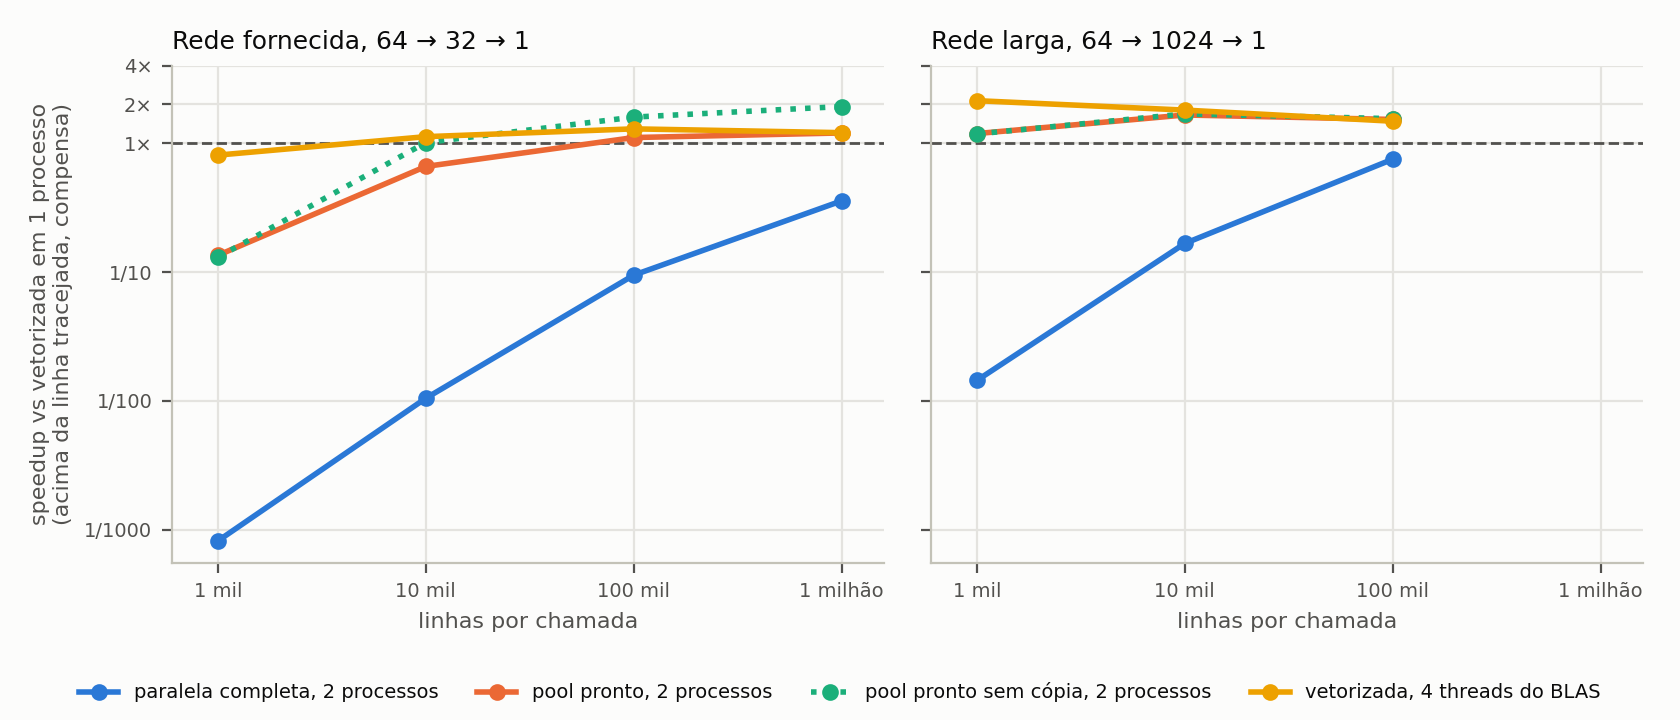
\includegraphics[width=0.62\linewidth]{speedup_por_linhas.png}
\caption{Speedup em relação à vetorizada, por número de linhas (escalas logarítmicas).}
\end{figure}

\section{Para onde vai o tempo}

\begin{enumerate}
\item \textbf{A referência escalar é lenta pelo interpretador, não pela conta.} A linha mais
  executada (2.080 vezes por observação) custa cerca de 151~ns: 85\% vão na leitura de
  elementos do array, um a um (cada leitura cria um objeto \texttt{numpy.float64}), e só 7\%
  na multiplicação e soma. Isso estima 314~\textmu s por observação; o medido foi 338~\textmu s.
  A vetorizada troca os laços por dois produtos de matrizes e é de 1.544 a 2.758\x{} mais
  rápida.
\item \textbf{Criar processos custa cerca de 120~ms fixos.} Com 1 mil linhas, em que os dados
  são desprezíveis, a paralela completa levou 123~ms com 2 processos e 126~ms com 4: é o
  tempo de iniciar um interpretador por filho, importar o NumPy e encerrar. Equivale a
  calcular cerca de 550 mil linhas na vetorizada.
\item \textbf{Validar e copiar os dados custa mais que o cálculo dividido.} Na
  Tabela~\ref{tab:cenarios}, com o pool já criado e X já na memória compartilhada, 2
  processos calculam 100 mil linhas em 9,6~ms; validar e copiar X soma 13,9~ms, e essa parte é
  serial, no processo pai.
\item \textbf{Não compensa nem com $n$ muito grande.} Entre 100 mil e 1 milhão de linhas,
  cada linha adicional custou 481~ns na paralela completa e 286~ns na vetorizada: alocar
  memória compartilhada nova e copiar X custam mais por linha do que o cálculo dividido
  economiza. Pela tendência, o speedup fica abaixo de 0,6\x{} (0,65\x{} com 4 processos); o
  maior valor medido foi 0,46\x, com 1 milhão de linhas.
\item \textbf{Entre as opções com processos, a memória compartilhada é a melhor.} Enviar cada
  lote de X por pickle, no mesmo pool já criado, foi de 5 a 7\x{} mais lento (133 contra
  25,8~ms com 100 mil linhas).
\end{enumerate}

\begin{table}[h]
\centering\small
\caption{Cenários com 100 mil linhas, em ms. As diferenças são medianas pareadas e agregam
várias parcelas.}
\label{tab:cenarios}
\begin{tabular}{rrrrrrr}
\toprule
Processos & Vetorizada & \cab{Pool pronto,\\sem cópia} & Pool pronto & Completa &
\cab{Validar e\\copiar X} & \cab{Criar processos e\\alocar memória} \\
\midrule
2 & 21,8 & 9,62 & 25,8 & 172 & 13,9 & 142 \\
4 & 21,8 & 6,72 & 20,0 & 175 & 13,3 & 155 \\
\bottomrule
\end{tabular}
\end{table}

\section{Extensões}

\begin{itemize}
\item \textbf{Lotes e 4 processos.} Com o pool pronto, 4 processos chegam a 1,12\x{} (100
  mil) e 1,57\x{} (1 milhão). Parte disso vem do lote: a própria vetorizada em lotes de
  4.096 linhas fica 1,37\x{} mais rápida com 1 milhão, porque deixa de alocar de uma vez um
  temporário $H$ de 256~MB. Com o mesmo lote nas duas, 2 processos empatam (1,38\x{} contra
  1,37\x) e 4 processos ganham cerca de 1,2\x. Lotes de 512 linhas geram até 1.954 tarefas e
  pioram: cada tarefa a mais custou de 10 a 17~\textmu s.
\item \textbf{Threads do BLAS, sem processos.} Aumentar o número de threads do OpenBLAS no
  próprio processo deu de 1,29 a 1,39\x{} com 2 threads e de 1,47 a 1,76\x{} com 4, a partir de
  10 mil linhas, sem cópia nem criação de processos: as threads leem o mesmo X.
\item \textbf{Fusão $y = Xw + b$.} São 64 multiplicações por linha em vez de 2.080: 2,9\x{}
  (5,6\x{} com 1 mil linhas). Preparar $w$ e $b$ leva 3,7~\textmu s e se paga na primeira
  chamada. A fusão reduz trabalho e não mede paralelismo; só vale enquanto não houver ativação
  entre as camadas.
\end{itemize}

\section{Recomendação}

Para este modelo, a vetorizada em um processo, em lotes de alguns milhares de linhas quando a
entrada é grande. Para mais vazão na mesma máquina, as threads do BLAS (até 1,76\x{} com 4).
Processos só compensam com o pool reutilizado e dados que já estejam na memória compartilhada
(de 2,1 a 4,0\x{} nesse cenário); criar processos a cada chamada não compensou em nenhum
tamanho. Enquanto o modelo for linear, a fusão das camadas dá cerca de 2,9\x{} com um único
processo e uma única thread.

\section{Limitações}

\begin{itemize}
\item Uma única VM compartilhada de 4 vCPUs: o pareamento protege as comparações, mas os
  tempos absolutos variam entre execuções. O teto de 0,6\x{} vem da tendência entre dois
  tamanhos.
\item O cenário ``pool pronto, sem cópia'' não valida nem copia as entradas: é um limite
  superior do ganho com processos, não uma estratégia completa, por isso passa de 2\x{} com 2
  processos.
\item A memória não foi medida (por construção, X existe duas vezes e cada filho só aloca o
  próprio lote), nem a referência escalar com 1 milhão de linhas (cerca de 6 minutos por
  chamada).
\end{itemize}

\end{document}
